% Бүлэг 1
\chapter{Улаанбаатар хотын дугуйн замын crowd-sourcing веб системийн тухай онол, арга зүйн судалгаа} % Бүлгийн нэр
\label{Chapter1} % Энэ бүлэг рүү ишлэл хийх бол \ref{Chapter1} командыг ашигла
%-------------------------------------------------------------------------------
% Агуулгад ашигласан хэвшүүлэлтийн зарим командын тодорхойлолт
\newcommand{\keyword}[1]{\textbf{#1}}
\newcommand{\tabhead}[1]{\textbf{#1}}
\newcommand{\code}[1]{\texttt{#1}}
\newcommand{\file}[1]{\texttt{\bfseries#1}}
\newcommand{\option}[1]{\texttt{\itshape#1}}
%-------------------------------------------------------------------------------
%-------------------------------------------------------------------------------
\section{Дугуйн замын мэдээллийн системийн тухай}
\paragraph{}
Газрын мэдээллийн систем /Geographic Information System, GIS/ нь газарзүйн байрлалтай холбоотой өгөгдлийг цуглуулах, хадгалах, боловсруулах, анализ хийх, газрын зураг дээр дүрслэх боломжийг олгодог мэдээллийн систем юм. GIS систем нь хот төлөвлөлт, зам тээвэр, байгаль орчны судалгаа зэрэг олон салбарт өргөн хэрэглэгддэг.
\begin{figure}[H]
    \centering
    % 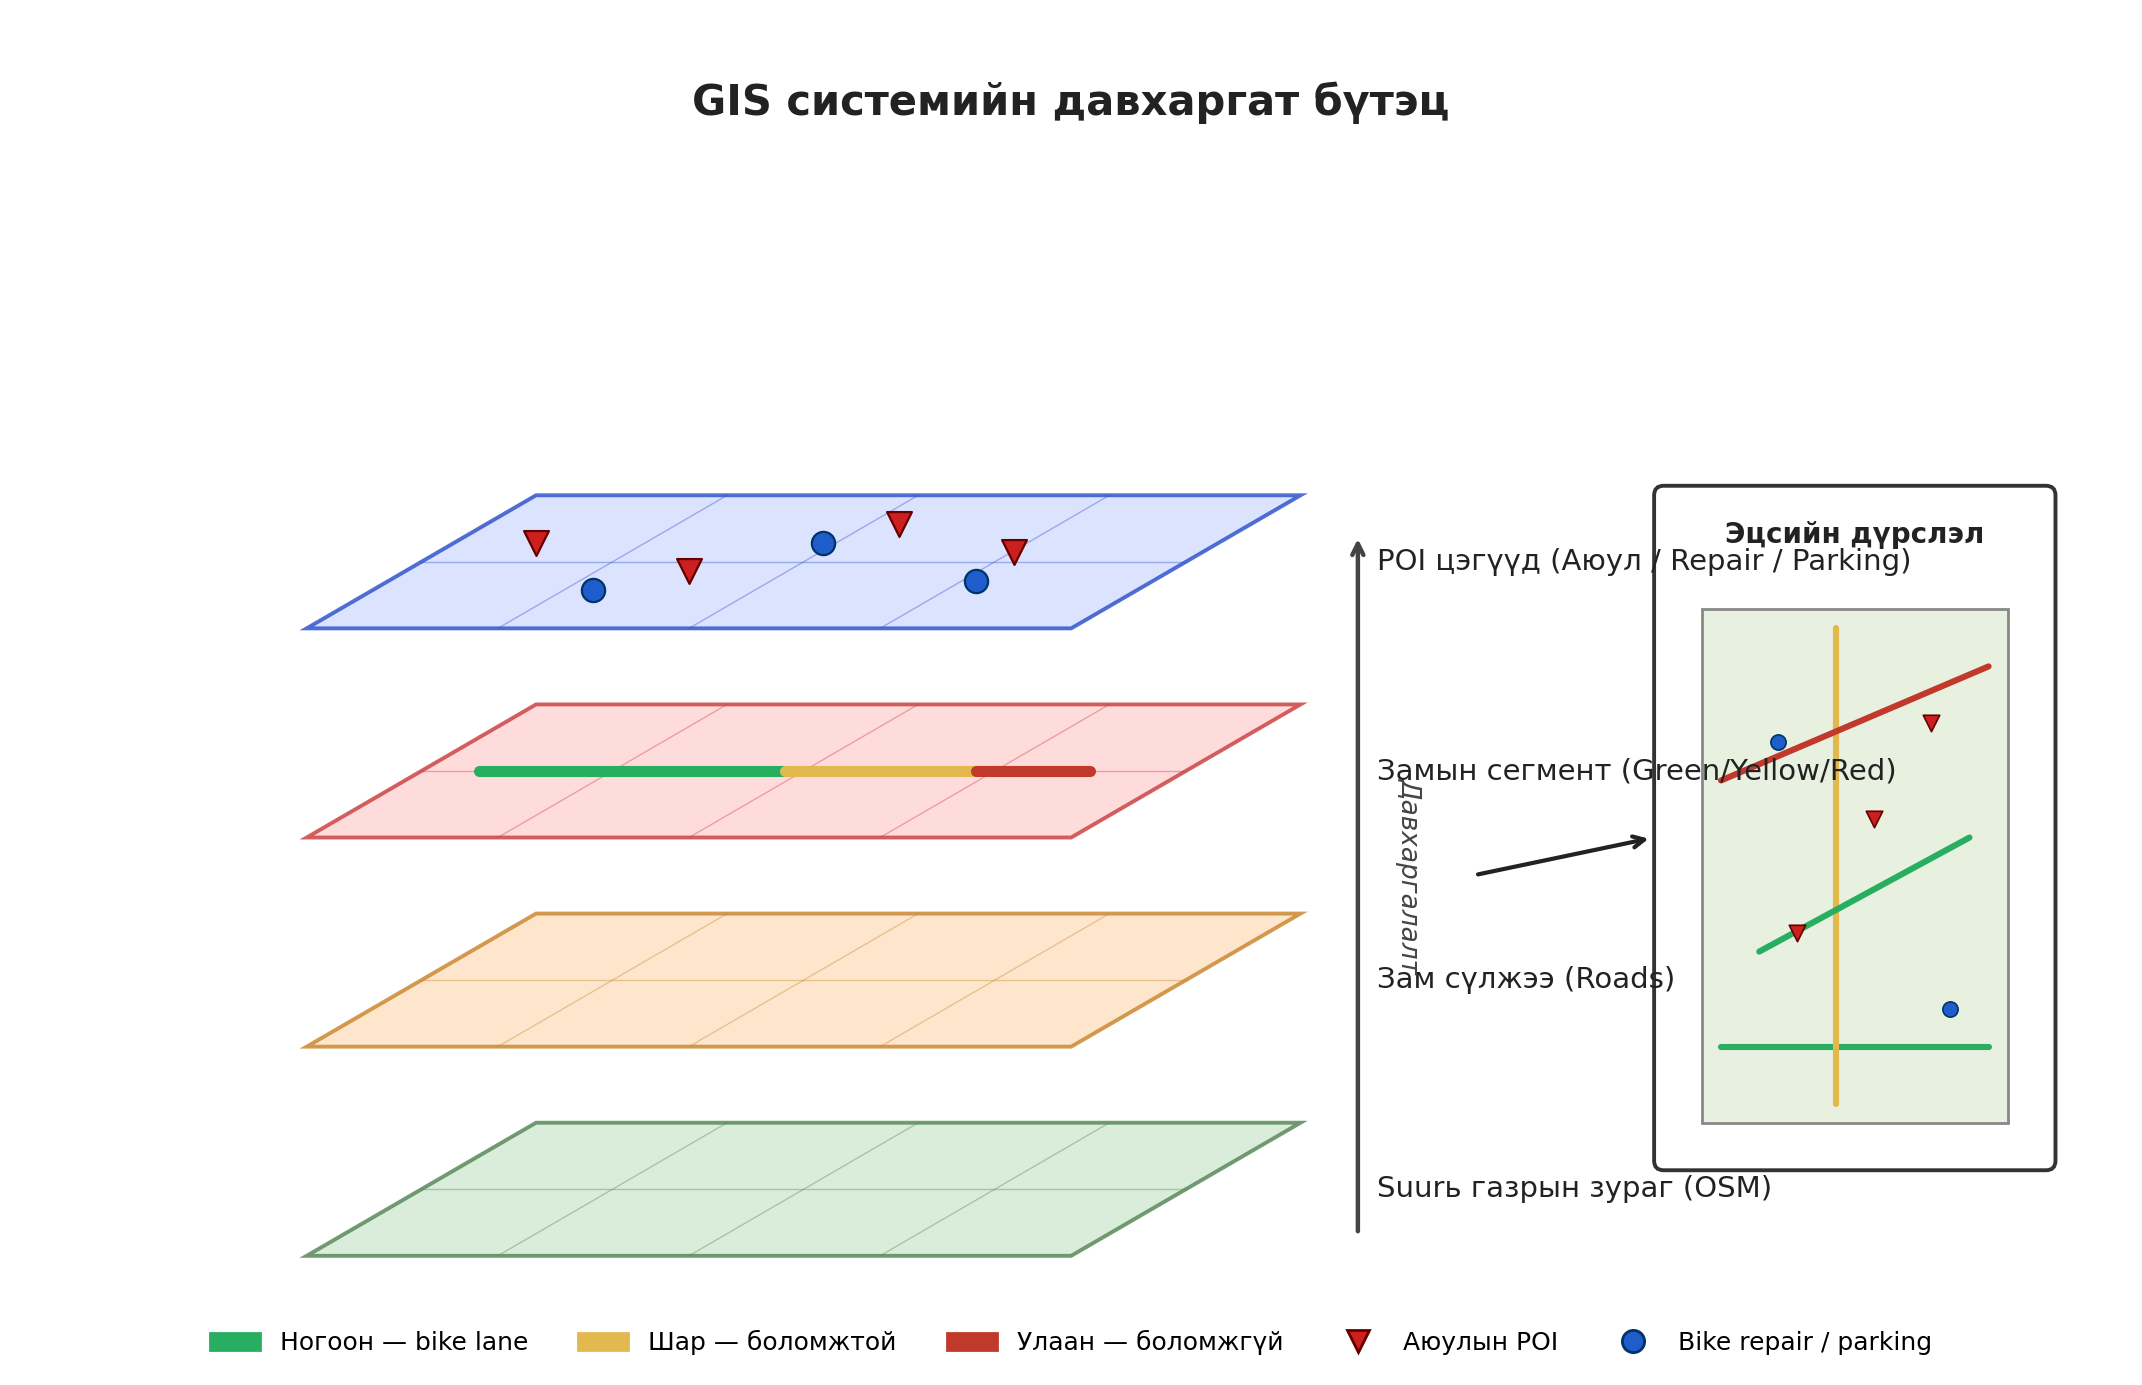
\includegraphics[scale=0.7]{Figures/chapter1/gis_example.png}
    \caption{GIS системийн өгөгдөл болон газрын зургийн дүрслэлийн жишээ}
    \label{fig:gis}
\end{figure}
Crowdsourcing систем нь олон хэрэглэгчийн оролцоонд тулгуурлан мэдээлэл цуглуулах арга бөгөөд хэрэглэгчид өөрсдийн өгөгдлийг системд оруулж, нийтлэг мэдээллийн сан бүрдүүлэх боломжийг олгодог. Энэхүү арга нь бодит цагийн, өргөн хүрээний мэдээллийг хурдан цуглуулах давуу талтай.
\begin{figure}[H]
    \centering
    % \includegraphics[scale=0.7]{Figures/chapter1/crowdsourcing.png}
    \caption{Crowdsourcing системийн ажиллагааны ерөнхий схем}
    \label{fig:crowd}
\end{figure}
Иймээс GIS болон crowdsourcing хосолсон систем нь дугуйн замын нөхцөл, аюулын мэдээллийг бодитой, динамик байдлаар тодорхойлох боломжийг бүрдүүлдэг. Хэрэглэгчид газрын зураг дээр замын сегмент тэмдэглэх, нөхцөл үнэлэх, сонирхолтой болон аюултай цэгүүдийг нэмэх замаар мэдээллийн санг баяжуулна.
%-------------------------------------------------------------------------------
\section{Ижил төстэй системийн судалгаа}
\paragraph{}
Дугуйн зам болон хөдөлгөөний мэдээллийг цуглуулах, визуалчлах чиглэлээр олон төрлийн системүүд хөгжсөн байдаг. Эдгээрээс Strava болон OpenStreetMap системүүдийг ижил төстэй системээр сонгон судлав.
\par \textbf{Strava аппликейшн :}
Strava нь GPS ашиглан хэрэглэгчийн явсан зам, хурд, хугацаа зэрэг мэдээллийг бүртгэж, газрын зураг дээр харуулдаг спорт аппликейшн юм.
\begin{figure}[H]
    \centering
    % \includegraphics[scale=0.4]{Figures/chapter1/strava.png}
    \caption{Strava аппликейшны GPS замын дүрслэл}
    \label{fig:strava}
\end{figure}
\par \textbf{OpenStreetMap систем :}
OpenStreetMap нь олон нийтийн оролцоонд тулгуурласан нээлттэй газрын зургийн платформ юм.
\begin{figure}[H]
    \centering
    % \includegraphics[scale=0.5]{Figures/chapter1/osm.png}
    \caption{OpenStreetMap газрын зургийн интерфейс}
    \label{fig:osm}
\end{figure}
\begin{longtable}{| p{7cm} | p{4cm} | p{4cm} |}
\caption{Судлагдсан системүүдийн харьцуулалт}
\label{tab:compare}\\
\hline
{\bfseries Системүүд } & {\bf Strava} & {\bf OpenStreetMap} \\ \hline
{\bf Платформын төрөл} & Мобайл апп & Веб апп \\ \hline
{\bf GPS зам бүртгэх} & Тийм & Хязгаарлагдмал \\ \hline
{\bf Crowdsourcing} & Тийм & Тийм \\ \hline
{\bf Замын нөхцөл үнэлэх} & Үгүй & Хязгаарлагдмал \\ \hline
{\bf POI нэмэх} & Үгүй & Тийм \\ \hline
{\bf Үнэгүй эсэх} & Хэсэгчлэн & Тийм \\ \hline
\end{longtable}
%-------------------------------------------------------------------------------
\section{Системийн үндсэн ойлголт}
\paragraph{}
Энэхүү систем нь дугуйн замын мэдээллийг олон хэрэглэгчээс цуглуулж, нэгтгэн боловсруулж, газрын зураг дээр харуулах crowdsourcing GIS систем юм.
\begin{figure}[H]
    \centering
    % \includegraphics[scale=0.7]{Figures/chapter1/system_overview.png}
    \caption{Системийн ерөнхий ажиллагааны бүтэц}
    \label{fig:system}
\end{figure}
Системийн үндсэн функцууд нь:
\begin{itemize}
    \item Газрын зураг дээр замын сегмент тэмдэглэх
    \item Замын нөхцлийг үнэлэх (ногоон, шар, улаан ангилал)
    \item Аюултай болон сонирхолтой цэгүүд (POI) нэмэх
    \item Бусад хэрэглэгчдийн мэдээллийг харах
\end{itemize}
Олон хэрэглэгчийн оруулсан өгөгдлийг нэгтгэх crowd aggregation аргаар тухайн замын бодит нөхцлийг тодорхойлно.
%-------------------------------------------------------------------------------
%   ХӨГЖҮҮЛЭЛТЭД АШИГЛАХ АЛГОРИТМ — BikeMap UB
%-------------------------------------------------------------------------------
\section{Хөгжүүлэлтэд ашиглах алгоритм}
\paragraph{} Энэ бүлэг нь системийн хөгжүүлэлтийн гол хэсэг болох \textit{Crowd Aggregation} (олон хэрэглэгчийн өгөгдлийг нэгтгэх) алгоритм болон \textit{Smart Route} (OSRM маршрут дээр аюулгүй байдлын давхарга нэмэх) алгоритмыг тайлбарлана.
%-------------------------------------------------------------------------------
\subsection{Crowd Aggregation алгоритм}
\paragraph{}
\textbf{Crowd Aggregation} буюу олон хэрэглэгчийн оруулсан замын нөхцлийн тэмдэглэгээг нэгтгэн тухайн сегментийн \emph{давамгай} (dominant) нөхцлийг тодорхойлох алгоритм нь системийн \textit{back-end} хэсгийн үндсэн логик болно. Уг алгоритм нь \texttt{apps/aggregation/tasks.py} файлд \texttt{update\_aggregation(segment)} функц хэлбэрээр хэрэгжсэн ба сегмент шинээр үүссэн эсвэл шинэчлэгдэх бүрд автоматаар дуудагдана.

\textbf{Зарчим:} Сегмент бүрт хэрэглэгчид {\color{green}$\bullet$}~(\textit{green}), {\color{olive}$\bullet$}~(\textit{yellow}), {\color{red}$\bullet$}~(\textit{red}) гэсэн гурван ангиллын аль нэгийг сонгон санал өгнө. Систем тухайн сегментийн орчинд (bounding box: $\pm 0.001$ градус $\approx 110$ метр) байрлах бүх сегментийн саналуудыг тоолж, хамгийн их санал авсан ангиллыг тухайн орон зайн нүдний \emph{давамгай нөхцөл} болгон тодорхойлно.

\textbf{Spatial hash:} Координатуудыг 3 оронтой тоогоор бөөрөнхийлж SHA-256 hash хийн \texttt{segment\_hash} (CHAR(64)) утга үүсгэнэ. 3 оронтой бөөрөнхийлөлт нь $\approx 110$ метрийн нарийвчлалыг өгдөг учир ойролцоо сегментүүд нэг hash утга авна.
\begin{equation}
\text{hash}(s) = \text{SHA256}\big(\text{round}(s_{\text{lat,lng}}, 3)\big)[:64]
\end{equation}

\textbf{Давамгай нөхцлийн тооцоолол:}
\begin{equation}
\text{dominant}(s) = \begin{cases}
\text{``none''}, & \sum_{c} V_c(s) = 0 \\
\arg\max\limits_{c \in \{green, yellow, red\}} V_c(s), & \text{бусад тохиолдолд}
\end{cases}
\end{equation}
Энд $V_c(s)$ нь $s$ сегментийн hash нүдэнд $c$ ангиллаар өгөгдсөн нийт саналын тоо.

\textbf{Жишээ:} $V_{green} = 10$, $V_{yellow} = 3$, $V_{red} = 6$ бол $\text{dominant} = green$ болно.

\textbf{Алгоритмын алхмууд:}
\begin{enumerate}
    \item Хадгалагдсан сегментийн координатаас \texttt{segment\_hash} тооцоолох
    \item Тухайн hash орон зайд (bounding box $\pm 0.001^{\circ}$) байрлах бүх сегментийг өгөгдлийн сангаас татах
    \item green / yellow / red тус бүрээр саналын тоог тоолох
    \item Нийт санал 0 бол \texttt{dominant = "none"}, бусад тохиолдолд хамгийн их саналтайг \texttt{dominant} болгох
    \item Үр дүнг \texttt{CrowdAggregation} хүснэгтэд \texttt{get\_or\_create()} -ээр шинэчилж хадгалах
\end{enumerate}
\begin{figure}[H]
    \centering
    % \includegraphics[width=0.9\textwidth]{Figures/chapter1/crowd-aggregation-architecture.png}
    \caption{Crowd Aggregation алгоритмын архитектур}
    \label{fig:crowdAgg}
\end{figure}
\begin{figure}[H]
    \centering
    % \includegraphics[width=0.9\textwidth]{Figures/chapter1/crowd-flow.png}
    \caption{Олон хэрэглэгчийн санал нэгтгэх процесс}
    \label{fig:crowd-flow}
\end{figure}
%-------------------------------------------------------------------------------
\subsection{Smart Route — Маршрутын аюулгүй байдлын визуалчлал}
\paragraph{}
\textbf{Smart Route} нь OpenStreetMap өгөгдөл дээр суурилсан \textbf{OSRM} серверийн \textit{cycling profile} -ийн маршрут дээр crowd aggregation болон POI өгөгдөлд тулгуурласан аюулгүй байдлын давхаргыг нэмж харуулдаг механизм юм. Уг механизм нь \texttt{apps/routes/views.py} файлын \texttt{SmartRouteView} класс дотор хэрэгжсэн.

OSRM нь \textit{Contraction Hierarchies} алгоритмаар богино зам тооцоолох (\textit{shortest cycling path}) даалгаврыг гүйцэтгэх бөгөөд Smart Route нь түүний үр дүн дээр crowd-sourcing өгөгдлөөр **annotation давхарга** нэмэхэд гол үүрэгтэй.

\textbf{Smart Route нь дараах 4 алхмаас бүрдэнэ:}
\begin{enumerate}
    \item \textbf{OSRM-аас үндсэн маршрут авах:}
    \begin{equation*}
    \mathit{GET}~\texttt{/route/v1/cycling/} \langle lng_1, lat_1 \rangle ; \langle lng_2, lat_2 \rangle
    \end{equation*}
    OSRM нь GeoJSON хэлбэрийн coordinate жагсаалт ($R = [(lng_i, lat_i)]_{i=1}^n$), \texttt{distance} (метр), \texttt{duration} (секунд) -ийг буцаана.
    \item \textbf{Сегмент бүрд crowd өнгийг тэмдэглэх:} Маршрут $R$ -ийн дараалсан хос цэг $(p_i, p_{i+1})$ -ийн орчинд (bounding box $\pm 0.002^{\circ}$) байрлах эхний \texttt{CrowdAggregation} -ийг хайж тухайн сегментэд $\text{colour}_i \in \{green, yellow, red, unknown\}$ утгыг оноох.
    \item \textbf{Аюулын POI -ийг илрүүлэх:} Маршрут дагуух цэг бүрийн ойролцоо ($\pm 0.0005^{\circ} \approx 55$м) байрлах баталгаажсан POI-уудаас \texttt{poi\_type} нь \{\texttt{danger, road\_damage, no\_bike\_lane}\} -д хамаарах объектуудыг буцаана. Давхардсан POI -г \texttt{set} -ээр шүүж нэг бүрд оруулна.
    \item \textbf{Front-end рүү буцаах:}
    \begin{equation*}
    \texttt{response} = \{ \text{mode}, \text{distance\_m}, \text{duration\_s}, R, \text{segments\_colour}, \text{hazards} \}
    \end{equation*}
\end{enumerate}

\textbf{Маршрутын төрлүүд:} API-н \texttt{mode} параметр \texttt{"safe"} эсвэл \texttt{"fast"} утга авна. Одоогоор хоёулангийнх нь үр дүн ижил буюу OSRM -ийн cycling profile -ийн санал болгосон зам байдаг (US-041 -ийн ирээдүйн өргөтгөлд safe-аар улаан сегментийг тойрсон альтернатив маршрут гаргахаар төлөвлөгдсөн).

\textbf{Алдааны хамгаалалт:} Хэрэв OSRM сервер хариу өгөхгүй (timeout, server down) бол систем шууд эхлэл, төгсгөлийг холбосон шулуун шугам (fallback line) -ыг \texttt{distance\_m=1000}, \texttt{duration\_s=300} утгуудтай буцаана.

\begin{figure}[H]
    \centering
    % \includegraphics[width=1\textwidth]{Figures/chapter1/smart-route-architecture.png}
    \caption{Smart Route алгоритмын архитектур}
    \label{fig:smartRoute}
\end{figure}
\begin{figure}[H]
    \centering
    % \includegraphics[width=0.9\textwidth]{Figures/chapter1/route-annotation.png}
    \caption{OSRM маршрут дээр crowd өнгө болон аюулын POI -г давхаргалсан байдал}
    \label{fig:route-annotation}
\end{figure}

%-------------------------------------------------------------------------------
\subsection{GPX Export алгоритм}
\paragraph{}
\textbf{GPX Export} (US-003) нь хэрэглэгчийн browser session-д цугласан GPS координатуудыг \textit{GPS Exchange Format} (.gpx) стандартын дагуу XML файл болгож хөрвүүлж буцаах механизм юм. \texttt{apps/routes/views.py} -ийн \texttt{GPXExportView} класс дотор Python -ийн стандарт сан болох \texttt{xml.etree.ElementTree} ашиглан хэрэгжүүлсэн.

\textbf{Алгоритмын алхам:}
\begin{enumerate}
    \item Front-end -ээс \texttt{coordinates} массив (\{lat, lng, timestamp\} объектууд) -ыг хүлээн авах
    \item GPX 1.1 стандартын root \texttt{<gpx>} элемент үүсгэх (\texttt{version="1.1"}, \texttt{xmlns="http://www.topografix.com/GPX/1/1"})
    \item \texttt{<metadata>} (нэр, цаг) болон \texttt{<trk> > <trkseg>} track segment үүсгэх
    \item Цэг тус бүрд \texttt{<trkpt lat="..." lon="...">} болон \texttt{<time>} элементийг нэмэх
    \item \texttt{Content-Type: application/gpx+xml} толгой бүхий HTTP response буцаах (\texttt{Content-Disposition: attachment} -аар татаж авах горим)
\end{enumerate}
Үр дүнгийн файлыг Strava, Google Maps, Komoot гэх мэт олон үйлчилгээнд импортлох боломжтой.

%-------------------------------------------------------------------------------
\section{Технологийн судалгаа}
\begin{figure}[H]
    \centering
    % \includegraphics[width=1\textwidth]{Figures/chapter1/system-architecture.png}
    \caption{BikeMap UB системийн ерөнхий архитектур}
    \label{fig:system-architecture}
\end{figure}
\paragraph{}
Системийн хөгжүүлэлтэд back-end болон front-end технологиудыг хослуулан ашигласан. Back-end -ийг Python хэлний \textbf{Django} веб фреймворк дээр REST API хэлбэрээр хөгжүүлэн, front-end -ийг \textbf{Django Templates} болон \textbf{Vanilla JavaScript} ашиглан Server-Side Rendering (SSR) хэлбэрээр гүйцэтгэсэн. Газрын зургийн дүрслэлд \textbf{Leaflet} болон \textbf{OpenStreetMap}, маршрутын тооцоололд \textbf{OSRM} -ийг ашигласан.
%-------------------------------------------------------------------------------
\subsection{Back-End хөгжүүлэлтэд ашиглах технологиуд}

\subsubsection{Django}
\textbf{Django} (хувилбар 4.2.9) нь Python хэл дээр бичигдсэн өндөр түвшний веб фреймворк бөгөөд ORM, authentication, admin panel зэрэг бэлэн шийдлүүдтэй. CSRF, XSS, SQL Injection -аас хамгаалах middleware-үүдтэй учраас аюулгүй байдлын NFR01 шаардлагыг хангана. Системд хэрэглэгчийн нэвтрэлт, сегмент, POI, crowd aggregation, GPX export -ын логикийг тус тусдаа Django app болгож (\texttt{apps/accounts}, \texttt{apps/segments}, \texttt{apps/pois}, \texttt{apps/aggregation}, \texttt{apps/routes}) зохион байгуулсан.

\subsubsection{Django REST Framework (DRF)}
\textbf{DRF} (3.14.0) нь Django -г суурь болгож REST API үүсгэхэд зориулагдсан хүчирхэг сан юм. Front-end -тэй JSON форматтай өгөгдөл солилцох, serializer ашиглан Python object -ийг JSON болгож хөрвүүлэх, ViewSet \& Router -ээр CRUD үйлдлийг хялбаршуулна. \texttt{django-filter} (23.5) -ийг REST API endpoint -уудад шүүлтүүр оруулахад ашигласан.

\subsubsection{Simple JWT}
\textbf{djangorestframework-simplejwt} (5.3.1) нь JSON Web Token (JWT) -т суурилсан stateless authentication механизмыг хэрэгжүүлдэг. Системд US-070, US-071 (нэвтрэлт ба RBAC) шаардлагуудыг хангахад ашигласан. Access token -ийн хүчинтэй хугацаа 60 минут, refresh token -ийн хүчинтэй хугацаа 7 хоног, refresh-rotation болон blacklist механизмтай.

\subsubsection{OSRM}
\textbf{OSRM /Open Source Routing Machine/} нь OpenStreetMap -ийн өгөгдөлд тулгуурласан, C++ хэл дээр бичигдсэн өндөр гүйцэтгэлтэй маршрут тооцоолох сервер юм. \textit{Contraction Hierarchies} алгоритм ашиглан хотын хэмжээний маршрутыг хэдхэн миллисекундэд тооцоолж чадна. BikeMap UB системд \texttt{cycling} profile -ийг ашиглах ба public OSRM demo сервер (\texttt{router.project-osrm.org}) -ийг туршилтын зориулалтаар \texttt{settings.OSRM\_BASE\_URL} орчны хувьсагчаар тохируулсан.

\subsubsection{PostgreSQL ба SQLite}
Системийн өгөгдлийн санд \textbf{PostgreSQL} -ийг production орчинд ашиглана. PostgreSQL нь нээлттэй эхийн SQL DBMS бөгөөд spatial өгөгдөл (POINT, LINESTRING) хадгалах, JSON баримтжуулалт, concurrent write зэрэг олон давуу талтай. Хөгжүүлэлтийн орчинд \textbf{SQLite} -ийг ашиглах бөгөөд \texttt{DATABASE\_URL} орчны хувьсагчаар PostgreSQL руу автоматаар шилжүүлэхээр \texttt{dj-database-url} (2.1.0) -ийг тохируулсан. PostgreSQL -ийн адаптерын \texttt{psycopg2-binary} (2.9.9) -ийг ашигласан.

\subsubsection{Gunicorn ба WhiteNoise}
\textbf{Gunicorn} (21.2.0) нь Python -ийн WSGI HTTP сервер бөгөөд production орчинд Django app -ийг ажиллуулахад ашигладаг. \textbf{WhiteNoise} (6.6.0) нь статик файлуудыг (CSS, JS, зураг) Django app -ийн дотроос шууд үйлчлэх боломжийг олгох сан бөгөөд тусдаа CDN тохируулахгүй cloud -д deploy хийхэд тохиромжтой. Heroku platform дээр \texttt{Procfile} -ээр Gunicorn -ийг WSGI сервер болгож ашиглана.

\subsubsection{Нэмэлт Python сангууд}
\begin{itemize}
    \item \textbf{django-cors-headers} (4.3.1) — Cross-Origin Resource Sharing (CORS) middleware
    \item \textbf{django-filter} (23.5) — REST API дээр шүүлтүүр оруулахад
    \item \textbf{Pillow} (10.2.0) — POI -д хавсаргах зургийн боловсруулалт (US-023)
    \item \textbf{python-dotenv} (1.0.1) — \texttt{.env} орчны хувьсагчдыг ачаалахад
    \item \textbf{requests} (2.31.0) — OSRM сервер рүү HTTP хүсэлт явуулахад
    \item \textbf{xml.etree.ElementTree} (Python стандарт сан) — GPX файл генерацид
\end{itemize}

\subsubsection{PyCharm}
\textbf{PyCharm} нь JetBrains компанийн хөгжүүлсэн Python -д зориулсан Integrated Development Environment (IDE). Django integration, database tool, debugger, code refactoring зэрэг функцуудтай. BikeMap UB системийн back-end хөгжүүлэлтэд ашигласан.

%-------------------------------------------------------------------------------
\subsection{Front-End хөгжүүлэлтэнд ашиглах технологиуд}

\subsubsection{Django Templates}
Front-end -ийн HTML markup -ийг \textbf{Django Template Engine} ашиглан Server-Side Rendering (SSR) хэлбэрээр гүйцэтгэсэн. Гол template файлууд нь \texttt{templates/base/base.html} (баазын layout), \texttt{templates/auth/login.html}, \texttt{register.html}, \texttt{profile.html}, \texttt{templates/map/index.html} (газрын зургийн нүүр), \texttt{templates/dashboard/index.html} (админы dashboard). Энэ хандлага нь React -тэй харьцуулахад жижиг бөгөөд хурдан, build алхамгүй, SEO -д ээлтэй давуу талтай.

\subsubsection{Vanilla JavaScript}
Front-end -ийн dynamic үйлдлүүдийг (\texttt{static/js/auth.js}, \texttt{static/js/api.js}) Vanilla JavaScript ашиглан хөгжүүлсэн. JWT токеныг localStorage -д хадгалах, REST API руу \texttt{fetch()} хүсэлт явуулах, Leaflet газрын зурагтай харьцах гэх мэт логикийг хариуцана. React, Vue гэх мэт фреймворкгүйгээр шууд browser -ийн API ашигласан нь bundle хэмжээг багасгах, ачаалал хурдасгах давуу талтай.

\subsubsection{Leaflet + OpenStreetMap}
\textbf{Leaflet} (1.9.4) нь BSD-2 License -тэй, JavaScript -ээр бичигдсэн интерактив газрын зургийн нээлттэй эхийн сан юм. Хэмжээ нь маш бага (\textasciitilde 42KB) бөгөөд гар утсан болон ширээний компьютерт зориулсан responsive газрын зургуудыг үүсгэх боломжийг олгоно. \textbf{OpenStreetMap} (OSM) -ийн tile -ийг ашиглан газрын зургийг үнэгүй, API key шаардахгүйгээр харуулна. Дараах онцлогуудыг ашиглана:
\begin{itemize}
    \item \texttt{L.map()} — газрын зураг үүсгэх
    \item \texttt{L.tileLayer()} — OSM tile layer
    \item \texttt{L.marker()} — POI -ийн marker байрлуулах
    \item \texttt{L.polyline()} — сегмент болон маршрутыг өнгөөр зурах
    \item \texttt{L.popup()} — POI дээр дарахад дэлгэрэнгүй харуулах
\end{itemize}

\subsubsection{Bootstrap 5 ба Bootstrap Icons}
\textbf{Bootstrap 5} (5.3.2) нь Twitter компанийн боловсруулсан, MIT License -тэй, нээлттэй эхийн front-end CSS фреймворк юм. Responsive (mobile-first) дизайны зарчимтай, 12-баганат grid system, бэлэн UI компонент (Button, Modal, Form, Card, Navbar) -тэй. CDN -ээс шууд ачааллах байдлаар ашигласан тул build алхам шаардахгүй. \textbf{Bootstrap Icons} (1.11.3) нь 1800+ үнэгүй икон агуулсан font icon сан бөгөөд navigation, кнопкууд, статусуудыг визуалчлахад хэрэглэгдэнэ.

\subsubsection{Visual Studio Code}
Front-end (HTML, JS, CSS) болон back-end (Python, Django template) хоёуланд нь \textbf{Visual Studio Code} -ийг ашигласан. Live Server, Prettier, ESLint, Django, Python (Pylance) гэх мэт өргөтгөлүүд нь хөгжүүлэлтийн бүтээмжийг нэмэгдүүлсэн.

%-------------------------------------------------------------------------------
\subsection{Кодын менежмент}
Системийн эх кодыг \textbf{GitHub} платформ дээр хадгалж, \textbf{Git} систем ашиглан хувилбар удирдлагыг гүйцэтгэсэн. Branching strategy: \texttt{main} (production), \texttt{develop} (active), \texttt{feature/*} (шинэ функц), \texttt{fix/*} (засвар). Pull Request механизмыг код шалгах (code review) -д ашигласан.

%-------------------------------------------------------------------------------
\section{Бүлгийн дүгнэлт}
\paragraph{}
Энэхүү бүлэгт BikeMap UB системийн үндсэн алгоритмууд болох Crowd Aggregation, Smart Route болон GPX Export алгоритмуудыг тодорхойлсон. Crowd Aggregation алгоритм нь олон хэрэглэгчийн оруулсан саналуудыг spatial hash -ээр бүлэглэн $\arg\max$ үйлдлээр давамгай нөхцлийг тооцдог энгийн ч найдвартай арга юм. Smart Route нь OSRM серверийн cycling маршрут дээр crowd aggregation -ээс гаргасан өнгөт давхарга болон ойролцоох аюулын POI -ийн жагсаалтыг хослуулсан annotation механизм бөгөөд OSRM сервер хариу өгөхгүй тохиолдолд fallback логиктой. GPX Export нь browser session-д цугласан GPS координатуудыг GPX 1.1 стандартын дагуу XML файл болгож буцаах боломжийг олгоно.

\paragraph{}
Мөн системийг хэрэгжүүлэхэд шаардлагатай технологиудыг судалж сонгосон. Back-end-д Python хэлний \textbf{Django 4.2.9} фреймворк, REST API-д \textbf{Django REST Framework 3.14.0}, JWT нэвтрэлтэд \textbf{Simple JWT 5.3.1}, өгөгдлийн санд \textbf{PostgreSQL} (production) болон \textbf{SQLite} (development), production server-д \textbf{Gunicorn 21.2.0} болон \textbf{WhiteNoise 6.6.0}, маршрут тооцоололд \textbf{OSRM} -ийг ашигласан. Front-end-д \textbf{Django Templates} болон \textbf{Vanilla JavaScript} -ийг хослуулан Server-Side Rendering хэлбэрээр гүйцэтгэж, газрын зургийн дүрслэлд \textbf{Leaflet 1.9.4} + \textbf{OpenStreetMap}, дизайнд \textbf{Bootstrap 5.3.2} + \textbf{Bootstrap Icons 1.11.3} -ийг ашигласан. Эдгээр технологиудын хослол нь системийн гүйцэтгэл (хөнгөн, build алхамгүй), өргөтгөх чадвар (cloud-friendly) болон хэрэглэгчийн туршлагыг (responsive UI) хангах боломжийг бүрдүүлж байна.
